\documentclass[A4,12PT, english, twocolumn]{journal}
\usepackage{amsmath,amssymb,amsfonts}
\usepackage[margin=0.7in]{geometry}
\usepackage{graphicx}
\usepackage{enumitem}
\usepackage{xcolor}
\usepackage{hyperref}
\usepackage{tabularray}
\usepackage{multicol}
\usepackage{tikz}
\usepackage{circuitikz}
\usepackage{scalerel}
\usepackage{pict2e}
\usepackage{tkz-euclide}
\usetikzlibrary{calc}
\usetikzlibrary{patterns,arrows.meta}
\usetikzlibrary{shadows}
\usetikzlibrary{external}

%pgfplots
\usepackage{pgfplots}
\pgfplotsset{compat=newest}
\usepgfplotslibrary{statistics}
\usepgfplotslibrary{fillbetween}

\def\infinity{\rotatebox{90}{8}}

% Hiperlink
\hypersetup{
    colorlinks=true,
    linkcolor=blue,
    filecolor=magenta,      
    urlcolor=cyan,
    pdftitle={Overleaf Example},
    pdfpagemode=FullScreen,
}
%\usepackage{style}
\NewDocumentCommand{\Log}{o}{%
\IfNoValueTF{#1}{}{{}^{#1}\!}\log}%
  
%command buat logaritma dengan basisnya di pojok kiri
%\textheight=17cm
%\textwidth=10cm
%\usepackage{blindtext}
\setenumerate[1]{itemsep=0,5cm}
\setenumerate[2]{topsep=5pt, itemsep=5pt, label=\textbf{\Alph*}.}

\title{Matematika Saintek \& Fisika UTUL UGM 2016 Kode 582}
\author{Fauzan Akbar Sukandar Putra \\ \LaTeX}

\begin{document}

\maketitle

%\begin{minipage}{0.5\textwidth}
\begin{enumerate}
%1%
\item Semua nilai $x$ yang memenuhi $|x+1| > x+3$ dan $|x+2| < 3$ adalah\dots
    \begin{enumerate}
        \item $x < -2$
        \item $-5 < x < -2$
        \item $x > -5$
        \item $-5 < x < 1$
        \item $x > 1$
    \end{enumerate}

%2%
\item Diketahui suku banyak $p(x)$ jika dibagi dengan $(x^2-2x)$ sisanya $(2-3x)$ dan jika dibagi $(x^2+x-2)$ sisanya $(x+2)$. Jika $p(x)$ dibagi dengan $(x^2-3x+2)$ maka sisanya adalah \dots
    \begin{enumerate}
        \item $x-10$
        \item $-x+10$
        \item $-7x-10$
        \item $7x-10$
        \item $-7x+10$
    \end{enumerate}

%3%
\item Jika $x_1$ dan $x_2$ memenuhi persamaan 
\begin{center}
    $\left( 2 \log{x-1} \right) \dfrac{1}{^x\log{10}} = \Log{10}$,
\end{center}
maka $x_1x_2 =$\dots
    \begin{enumerate}
        \item $5\sqrt{10}$
        \item $4\sqrt{10}$
        \item $3\sqrt{10}$
        \item $2\sqrt{10}$
        \item $\sqrt{10}$
    \end{enumerate}

%4%
\item Diketahui $x_1$ dan $x_2$ merupakan akar-akar $4x^2-7x+p=0$ dengan $x_1<x_2$. Jika $^2\log{\left( \frac{1}{3}x_1 \right)} = -2= \, ^2\log{x_2}$, maka $4x_1+x_2=$\dots
    \begin{enumerate}
        \item $\frac{19}{4}$
        \item $4$
        \item $\frac{15}{4}$
        \item $\frac{13}{4}$
        \item $3$
    \end{enumerate}

%5%
\item Luas daerah yang dibatasi oleh kurva $y= 2\cos{x}, \; y=1,$ sumbu $X$ dan sumbu $Y$ adalah\dots
    \begin{enumerate}
        \item $\frac{\pi}{6} = \int_{\frac{\pi}{3}}^{\frac{\pi}{2}} 2\cos{x} \, dx$
        \item $\frac{\pi}{3} = \int_{\frac{\pi}{6}}^{\frac{\pi}{2}} 2\cos{x} \, dx$
        \item $\frac{\pi}{3} = \int_{\frac{\pi}{3}}^{\frac{\pi}{2}} 2\cos{x} \, dx$
        \item $\frac{\pi}{2} = \int_{\frac{\pi}{3}}^{\frac{\pi}{2}} 2\cos{x} \, dx$
        \item $\frac{\pi}{2} = \int_{\frac{\pi}{6}}^{\frac{\pi}{2}} 2\cos{x} \, dx$
    \end{enumerate}

%6%
\item Empat siswa laki-laki dan tiga siswa perempuan berdiri di dalam suatu barisan. Banyaknya cara agar ketiga siswa perempuan berdampingan di barisan tersebut adalah\dots
    \begin{enumerate}
        \item $720$
        \item $360$
        \item $144$
        \item $72$
        \item $48$
    \end{enumerate}

%7%
\item Untuk suatu sudut $x$ dan $y$ berlaku
\begin{center}
    $\sin^2{x} + \cos^2{y} = \frac{3}{2}a$ \\
    $\cos^2{x} + \sin^2{y} = \frac{1}{2} a^2$
\end{center}
Jumlah semua nilai $a$ yang mungkin untuk sistem persamaan di atas adaah\dots
    \begin{enumerate}
        \item $-5$
        \item $-4$
        \item $-3$
        \item $3$
        \item $4$
    \end{enumerate}

%8%
\item Diketahui $10, \; x_2, \; x_3, \; x_4$ membentuk barisan geometri. Jika $x_2 - 10, \; x_3 - 10$ dan $x_4 - x_3 - x_2 - 10$ membentuk barisan aritmatika, maka nilai $x_4$ adalah\dots
    \begin{enumerate}
        \item $\frac{10}{27}$
        \item $\frac{5}{4}$
        \item $80$
        \item $270$
        \item $640$
    \end{enumerate}

%9%
\item Jika $a, \; 4, \; b$ adalah tiga suku berurutan dari barisan aritmatika dan $a, \; 3, \; b$ merupakan tiga suku berurutan suatu barisan geometri, maka $\frac{1}{a} + \frac{1}{b} =$\dots
    \begin{enumerate}
        \item $\frac{1}{4}$
        \item $\frac{1}{2}$
        \item $\frac{3}{4}$
        \item $\frac{8}{9}$
        \item $\frac{9}{8}$
    \end{enumerate}

%10%
\item $\lim\limits_{x \longrightarrow 3} \dfrac{\left(x+6 \right) \tan{\left(2x-6 \right)}}{x^2-x-6}=$\dots
    \begin{enumerate}
        \item $-\frac{18}{5}$
        \item $-\frac{9}{5}$
        \item $\frac{9}{5}$
        \item $\frac{18}{5}$
        \item $\frac{27}{5}$
    \end{enumerate}

%11%
\item Jika fungsi $g(x) = p \sqrt{x^2-4}$ naik pada $\left\{x \in \mathbb{R} | x \leq -2 \right \}$ dan turun pada $\left \{x \in \mathbb{R} | x \geq 2 \right \}$, maka himpunan semua nilai $p$ yang memenuhi adalah\dots
    \begin{enumerate}
        \item $\emptyset$
        \item $\left\{ p \in \mathbb{R} | p \geq 2 \right\}$
        \item $\left\{ p \in \mathbb{R} | p > 0 \right\}$
        \item $\left\{ p \in \mathbb{R} | p < 0 \right\}$
        \item $\left\{ p \in \mathbb{R}| p \leq -2 \right\}$
    \end{enumerate}
    
%12%
\item Diketahui titik $(1,p)$ berada pada lingkaran $x^2 + y^2 -2y = 0$. Persamaan lingkaran dengan pusat $(1,p)$ dan menyinggung garis $px + y = 4$ adalah\dots
    \begin{enumerate}
        \item $x^2 + y^2 -2x -2y - 2 = 0$
        \item $x^2 + y^2 -2x -2y - 1 = 0$
        \item $x^2 + y^2 -2x -2y = 0$
        \item $x^2 + y^2 -2x +2y - 2 = 0$
        \item $x^2 + y^2 -2x +2y - 1 = 0$
    \end{enumerate}

%13%
\item Jika $0 < x < \frac{\pi}{2}$ dan $2 \sin^2{x} + \cos^2{x} = \frac{34}{25}$ maka nilai $\tan{x}=$\dots
    \begin{enumerate}
        \item $-\frac{3}{4}$
        \item $-\frac{3}{5}$
        \item $\frac{3}{4}$
        \item $\frac{3}{5}$
        \item $\frac{4}{5}$
    \end{enumerate}

%14%
\item Diketahui vektor $OA=(1,2)$ dan vektor $OB=(2,1)$. Jika titik $P$ terletak pada $AB$ sehingga $AP : PB = 1 : 2$, maka panjang vektor $OP$ adalah\dots
    \begin{enumerate}
        \item $\frac{3}{2} \sqrt{2}$
        \item $\frac{1}{3} \sqrt{2}$
        \item $\frac{2}{3} \sqrt{2}$
        \item $\frac{1}{3} \sqrt{41}$
        \item $\frac{3}{2} \sqrt{41}$
    \end{enumerate}

%15%
\item Limas segiempat beraturan $T.ABCD$ mempunyai tinggi sama dengan dua kali panjang sisi $ABCD$. Jika titik $E$ berada pada garis $BC$ dengan $BE : EC = 1 : 1$ dan titik $F$ berada pada garis $TE$ dengan $TF : FE = 1 : 3$, maka panjang proyeksi $FE$ pada $ABCD$ adalah\dots kali sisi $ABCD$.
    \begin{enumerate}
        \item $\frac{9}{8}$
        \item $\frac{5}{8}$
        \item $\frac{4}{8}$
        \item $\frac{3}{8}$
        \item $\frac{1}{8}$
    \end{enumerate}
    

%FISIKA %
%16%
\newpage
\item Benda bermassa $2 \; kg$, dari keadaan diam dipercepat oleh gaya konstan sebesar $2 \; N$. Berapa waktu yang diperlukan oleh gaya tersebut sehingga benda bergerak dengan tenaga kinetik $100 \; J$.
    \begin{enumerate}
        \item $2 \; s$
        \item $4 \; s$
        \item $6 \; s$
        \item $8 \; s$
        \item $10 \; s$
    \end{enumerate}
  
%17%
\item Sebuah batu dilemparkan vertikal ke atas dari tanah dengan kecepatan awal $v_1$. Saat batu berada pada titik tertinggi, sebuah bola delemparkan juga ke atas dari tanah dengan kecepatan awal $v_2$. Ternyata batu dan bola menyentuh tanah secara bersamaan. Perbandingan tinggi maksimum batu dan bole adalah\dots
    \begin{enumerate}
        \item $16$
        \item $9$
        \item $4$
        \item $3$
        \item $2$
    \end{enumerate}
     
%18%
\item Sistem $2$ benda seperti gambar di bawah, diketahui bahwa bidang licin sempurna dan besar percepatan gravitasi setempat $g$. Kedua benda tersebut akan bergerak dengan percepatan sebesar\dots
\begin{center}
    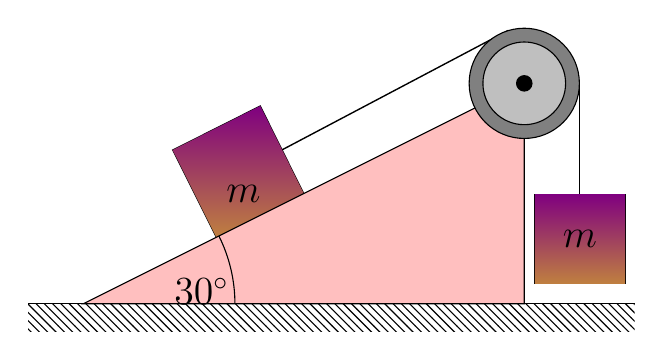
\begin{tikzpicture}[scale=0.70]
    %GRID
    %\draw[lightgray] (0,0) grid (10,10);
    %KOORDINAT
    \coordinate (A) at (0,0);
    \coordinate (B) at (8,0);
    \coordinate (C) at (8,4);
    %LANTAI
    \fill[pattern=north west lines] (-1,0) rectangle (10,-0.5);
    \draw (-1,0) -- (10,0);
    %TALI
    \draw[line width=0.5pt] (3.6,2.79) -- (7.71,4.96);
    \draw[line width=0.5pt] (9,4) -- (9,1.5);
    %KOTAK 1
    \draw[] (2.41,1.21) -- (4,2) -- (3.21,3.59) -- (1.62,2.79) -- (2.41,1.21);
    \shade[top color=violet, bottom color=brown] (2.41,1.21) -- (4,2) -- (3.21,3.59) -- (1.62,2.79) -- (2.41,1.21) node [midway, above=10pt, right=8pt]{\Large $m$};
    %KOTAK 2
    \draw[] (8.19,0.37) rectangle (9.83,1.99);
    \shade[top color=violet, bottom color=brown] (8.19,0.37) rectangle (9.83,1.99) node[midway]{\Large $m$};
    %SEGITIGA
    \draw[fill=pink] (A) -- (B) -- (C) -- cycle;
    %SUDUT
    \tkzMarkAngle[size=2.75](B,A,C);
    \tkzLabelAngle[above=3pt, right=10pt](B,A,C){\Large $30^\circ$};
    %LINGKARAN
    \draw[fill=gray] (C) circle (1cm);
    \draw[fill=lightgray] (C) circle (0.75cm);
    \fill[fill=black] (C) circle (0.15cm);
    \end{tikzpicture}
\end{center}
    \begin{enumerate}
        \item $g$
        \item $\frac{1}{2}g$
        \item $\frac{1}{3}g$
        \item $\frac{1}{4}g$
        \item $\frac{1}{5}g$
    \end{enumerate}
   
%19% 
\item Dua buah balok dengan massa $3 \; kg$ dan $4 \; kg$ ditumpuk dengan balok bermassa lebih kecil berada di atas. Kedua balok berada di atas lantai yang kasar dengan koefisien gesek antara lantai dan balok dan antara balok dan balok sama, yaitu koefisien gesek statik $0,3$ dan koefisien gesek kinetik $0,2$. Pada balok yang berada paling bawah diberi gaya arah horizontal sebesar $10 \; N$. Maka total gaya yang bekerja pada balok yang paling atas adalah\dots$N$
    \begin{enumerate}
        \item $-1,2$
        \item $-0,7$
        \item $0$
        \item $0,7$
        \item $1,2$
    \end{enumerate}
    
%20%
\item Sebuah bola pejal bermassa $m$ dan berjari-jari $R$ menggelinding pada bidang horizontal tanpa slip. Kemudian bidang horizontal tersebut bersambung dengan dasar bidang miring yang sudutnya $\theta$. Ketika bola mulai naik ke atas bidang miring, kecepatan awalnya $v_0$. Asumsikan gerak bola menaiki bidang miring tanpa slip, jarak terjauh yang ditempuh pada bidang miring adalah\dots
    \begin{enumerate}
        \item $\frac{7}{10} \frac{v_0^2}{g}$
        \item $\frac{7}{10} \frac{v_0^2}{g \sin{\theta}}$
        \item $\frac{7}{10} \frac{v_0^2}{g \cos{\theta}}$
        \item $\frac{10}{7} \frac{v_0^2}{g \sin{\theta}}$
        \item $\frac{10}{7} \frac{v_0^2}{g \cos{\theta}}$
    \end{enumerate}

%21%
\item Dua buah termometer $A$ dan $B$ masing-masing menunjuk angka $20^\circ$ dan $30^\circ$ untuk es mencair serta $180^\circ$ dan $230^\circ$ untuk air mendidih. Kedua termometer tersebut menunjuk angka suhu yang sama pada suhu termometer celcius sebesar\dots
    \begin{enumerate}
        \item $-10^\circ \; C$
        \item $-15^\circ \; C$
        \item $-20^\circ \; C$
        \item $-25^\circ \; C$
        \item $-30^\circ \; C$
    \end{enumerate}
    
%22% 
\item Sebanyak $m \; gram$ air bersuhu $4^\circ \; C$ dicampur dengan $n \; gram$ es bersuhu $-4^\circ \; C$. Ternyata keadaan akhir adalah setengah bagian es mencair. Perbandingan $m$ dan $n$ adalah\dots
    \begin{enumerate}
        \item $1:1$
        \item $1:2$
        \item $1:4$
        \item $2:1$
        \item $4:1$
    \end{enumerate}

%23%
\item Gas $A$ dan gas $B$ tersusun atas molekul-molekul diatomik. Massa molekul gas $A$ adalah 4 kali massa gas $B$. Dengan menganggap gas $A$ dan gas $B$ sebagai gas ideal, rasio energi kinetik rerata molekul gas $A$ terhadap molekul gas $B$ pada temperatur kamar adalah\dots
    \begin{enumerate}
        \item $1:1$
        \item $1:2$
        \item $1:\sqrt{2}$
        \item $1:\sqrt{3}$
        \item $1:4$
    \end{enumerate}
    
%24%  
\item Sebuah pipa logam yang cukup tipis memiliki jari-jari $a$. Pipa tersebut cukup panjang dan dialiri arus senilai $i$. Induksi magnetik di titik $P$ yang terletak sejauh $r$ dari sumbu pipa dengan $r>a$ adalah\dots
	\begin{enumerate}
		\item nol
		\item $\frac{\mu_0 i}{2 \pi r}$
		\item $\frac{\mu_0 i}{2 \pi (a-r)}$
		\item $\frac{\mu_0 i}{\pi r^2}$
		\item $\frac{\mu_0 i r}{\pi a^2}$
	\end{enumerate}

%25%
\item Kapasitor plat paralel dengan jarak kedua platnya $d$ dan kapasitansinya $C$, diisi muatan $Q$ sehingga potensialnya $V$. Muatan titik $q$ yang diletakkan di dalam kapasitor tersebut mengalami gaya elektrostatik sebesar\dots
   \begin{enumerate}
        \item $\frac{qQ}{d^2}$
        \item $\frac{qV}{d}$
        \item $\frac{qV}{C}$
        \item $qCV$
        \item $\frac{qQ^2}{C}$
   \end{enumerate}
   
%26%
\item Selembar plat dengan luas $A$ memiliki muatan senilai $Q$ yang tersebar merata. Kuat medan listrik di titik-titik yang sangat dekat dengan permukaan plat itu dan jauh dari sisi-sisinya adalah\dots
    \begin{enumerate}
        \item $\frac{2 \pi k Q }{A}$
        \item $-\frac{2 \pi k Q }{A}$
        \item $\frac{\pi k Q }{A}$
        \item $-\frac{\pi k Q }{A}$
        \item $\frac{k Q }{A}$
    \end{enumerate}
  
%27%  
\item Tinjau suatu rangkaian listrik sebagaimana ditunjukkan pada gambar. Hitunglah arus listrik $I_3$ dalam hambatan $2\Omega$.
\begin{center}
    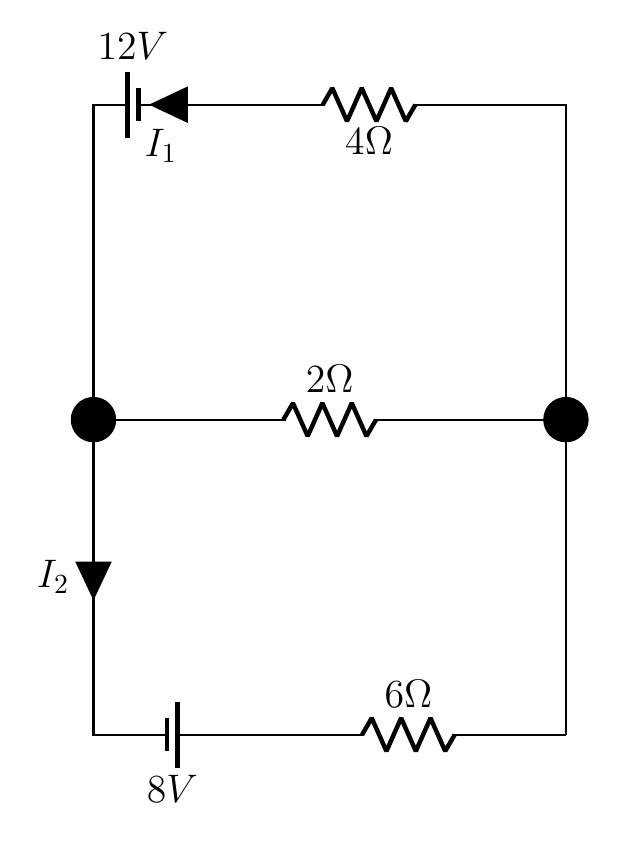
\begin{tikzpicture}
        %GRID
        %\draw[lightgray] (0,0) grid (6,8);
        %KOORDINAT
        \coordinate (A) at (6,0);
        \coordinate (B) at (0,0);
        \coordinate (C) at (0,4);
        \coordinate (D) at (0,8);
        \coordinate (E) at (6,8);
        \coordinate (F) at (6,4);
        %tangkaian
        \draw[thick] (6,0) to[resistor, a=\Large $6\Omega$] (2,0) to[battery1, l=\Large $8V$] (B) -- node[currarrow, sloped, pos=0.5, scale=3, xscale=-1]{} node[midway,left=5pt]{\Large $I_2$} (C) -- (D) to[battery1, a^=\Large $12V$] node[currarrow, sloped, pos=1, scale=3, xscale=-1]{} node[midway, below=5pt]{\Large $I_1$} (1,8) to [resistor, a=\Large $4\Omega$] (E) -- (F) -- (A);
        \draw[thick] (F) to[resistor, a=\Large $2\Omega$] (C);
        \draw[fill=black] (F) circle (8pt);
        \draw[fill=black] (C) circle (8pt);
    \end{tikzpicture}
\end{center}
    \begin{enumerate}
        \item $0.91 \; A$
        \item $0.61 \; A$
        \item $0.091 \; A$
        \item $0.061 \; A$
        \item $0 \; A$
    \end{enumerate}

%28%  
\item Sebuah partikel bermuatan $q$ dan bermassa $m$ bergerak dalam lintasan lingkaran dengan jari-jari $r$ dalam medan magnet serbasama $B$. Jika arah gerak partikel tegak lurus terhadap arah medan magnetik, hitunglah momentum partikel.
    \begin{enumerate}
        \item $qB^2r$
        \item $qBr^2$
        \item $qBr$
        \item $\frac{qB}{r}$
        \item $\frac{q^2B}{r}$
    \end{enumerate}

%29%  
\item Benda bermassa $2 \; kg$ bergetar selaras sederhana. ketika benda tersebut berada pada titik setimbang kecepatannya $2 \; m/s$ dan ketika di simpangan $20 \; cm$ benda itu diam. Kecepatan benda ketika di simpangan $16 \; cm$ sebesar\dots
    \begin{enumerate}
        \item $1,8 \; m/s$
        \item $1,6 \; m/s$
        \item $1,2 \; m/s$
        \item $1,0 \; m/s$
        \item $0,8 \; m/s$
    \end{enumerate}

%30%
\item Suatu pegas dengan konstanta pegas $k$ diregangkan sebesar $x$. Seandainya separuh usaha yang digunakan untuk meregangkan pegas tadi dipakai untuk meregangkan pegas kedua, pegas kedua ternyata teregang sebesar $\frac{x}{4}$. Maka konstanta pegas kedua adalah \dots k 
    \begin{enumerate}
        \item $2$
        \item $4$
        \item $6$
        \item $8$
        \item $32$
    \end{enumerate}
 
%31%
\item Pada cermin cekung dengan jarak fokus $f$, jika perbesaran yang dihasilkan adalah $n\left( n > 1 \right)$, maka jarak antara benda dengan bayangan dapat dituliskan sebagai\dots
    \begin{enumerate}
        \item $\left( \frac{n+1}{n} \right) f$
        \item $\left( n+1 \right) f$
        \item $\left( \frac{n^2-1}{n^2+1} f \right)$
        \item $\left( \frac{n^2+1}{n} f \right)$
        \item $\left( \frac{n^2-1}{n} f \right)$
    \end{enumerate}

%32%
\item Sebuah batang panjang diamnya $L$. Batang tersebut bergerak searah dengan arah membujurnya, sehingga dilihat oleh pengamat yang diam panjangnya adalah $0,6L$. Pengamat lain yang bergerak searah dengan gerak batang, mengamati panjang batang sebesar $0,8L$. Jika $c$ adalah kelajuan cahaya, maka kelajuan batang relatif terhadap pengamat yang bergerak adalah\dots
    \begin{enumerate}
        \item $0,8 \; c$
        \item $0,6 \; c$
        \item $0,5 \; c$
        \item $0,4 \; c$
        \item $0,2 \; c$
    \end{enumerate}

%33%
\item Suhu suatu permukaan benda hitam adalah $693^\circ \; C$. Intensitas maksimum yang dipancarkan oleh permukaan benda tersebut terjadi pada frekuensi\dots
    \begin{enumerate}
        \item $2 \times 10^14 \; Hz$
        \item $10^14 \; Hz$
        \item $5 \times 10^13 \; Hz$
        \item $2 \times 10^13 \; Hz$
        \item $10^13 \; Hz$
    \end{enumerate}

%34%
\item Sebuah partikel bermassa $M$ meluruh dari keadaan diam menjadi dua partikel, yang satu bermassa $m$ dan yang satu lagi tidak bermassa. Besar momentum partikel yang bermassa $m$ adalah\dots
    \begin{enumerate}
        \item $\frac{\left( M^2-2m^2 \right)c}{M}$
        \item $\frac{\left( 2M^2-m^2 \right)c}{M}$
        \item $\frac{m^2c}{M}$
        \item $\frac{M^2c}{M}$
        \item $\frac{\left( M^2-m^2 \right)c}{2M}$
    \end{enumerate}

%35%
\item Sebuah roket bermassa $m$ bergerak ke atas permukaan planet bermassa $M$ berjari-jari $R$ dengan kecepatan awal $\frac{1}{2}$ kali kecepatan lepas. Tinggi maksimum roket dari permukaan planet adalah\dots
    \begin{enumerate}
        \item $\frac{4}{3}R$
        \item $R$
        \item $\frac{2}{3}R$
        \item $\frac{1}{2}R$
        \item $\frac{1}{3}R$
    \end{enumerate}

\end{enumerate}
\end{document}  
